\chapter{设置线条类型和标记类型的显示样式\label{ch09}}
在 matplotlib 的大量实践中,会频繁地进行折线图的线条类型和标记类型的设置工作。更加重要的是,线条类型和标记类型的显示样式的美观与否会极大地影响 Python 数据可视化的效果。

这部分会涉及字典数据结构作为关键字参数的使用方法、线条类型的设置方法和标记类型的设置方法。
\section{不同调用签名形式的字典使用方法}
在 Python 数据可视化的代码实现中,大量运用了字典数据结构。\textbf{在函数或是实例方法的调用签名中,字典数据结构经常作为关键字参数值进行调用而传入代码块中。}通过使用字典设置相应属性的属性值,大大提高了代码的简洁程度,并减少了重复设置的烦琐工作。
\section{线条类型的显示样式设置方法}
在折线图中,我们通过函数或是实例方法 plot() 的关键字参数 linestyle(ls) 设置线条类型的显示样式。
\section{标记类型的显示样式设置方法\label{193}}
\begin{figure}
    \centering
    \caption{标记类型的显示样式}
    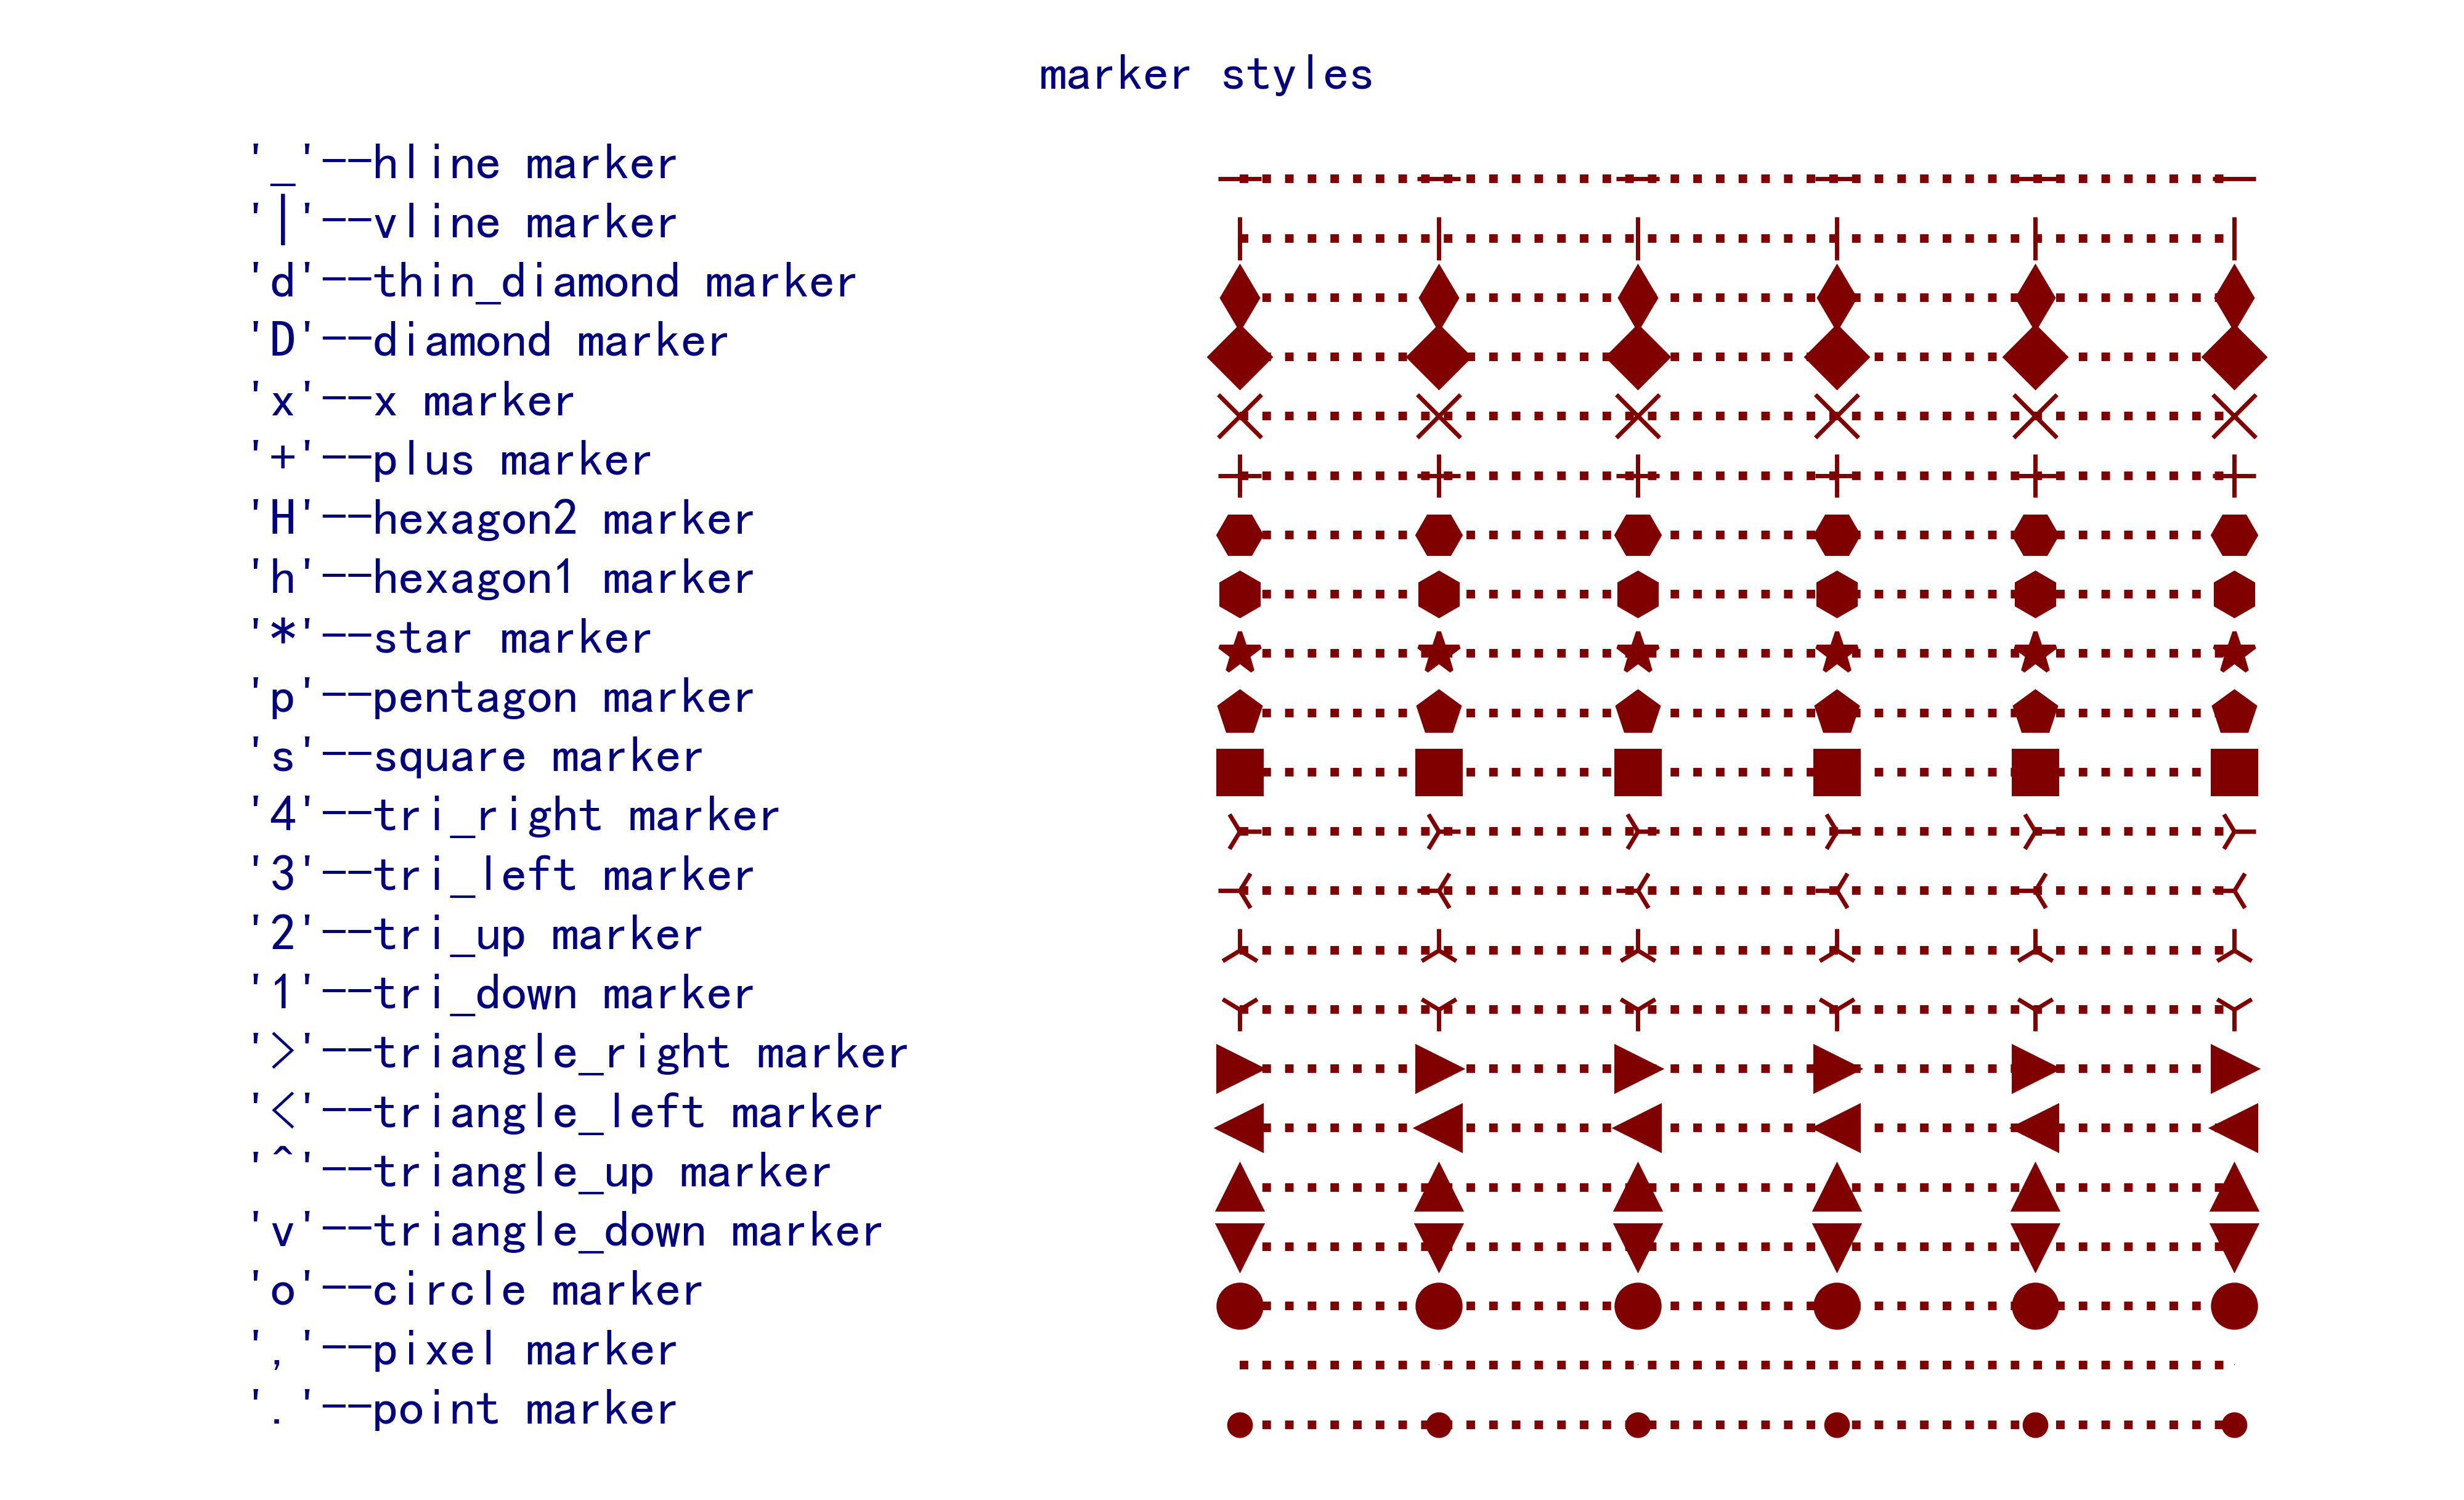
\includegraphics{9787121348884/img/fig9-4.png}
\end{figure}
\section{延伸阅读}
\subsection{“破折号”线条样式的不同展现形式的设置方法}
线条类型是“破折号”样式的折线呈现多种展现形式,实现多种展现形式的关键是关键字参数 dashes 的使用。折线是由若干个数据点所组成的,如果我们将这些数据点中的一些数据点有规律地抹掉,就会出现“破折号”样式的折线。因此,控制数据点的抹去模式就可以实现“破折号”样式的折线的多种展现形式。

语句
\begin{verbatim}
    ax.plot(x, y + 0.4, dashes=[2, 2, 8, 2])
\end{verbatim}
里的关键字参数 dashes 的取值含义是:折线组成单元是由 2 个数据点的线段、2 个数据点的间隔、8 个数据点的线段和 2 个数据点的间隔所组成的结构单元。

\subsection{标记填充样式的设置方法}
\nameref{193}已经介绍过有关标记类型的显示样式的相关内容。现在,我们再进一步考虑标记样式能否通过标记填充样式得以展现,也就是说,借助标记填充样式的选择也可以同样实现标记显示样式的设置需求,而且同种标记类型会由于标记填充样式的不同而呈现出更加丰富的展示效果,这就极大地丰富了标记展示样式的内容。
\subsection{函数 plot() 的调用签名的设置方法}
函数 plot() 用来绘制有序数对的折线和标记的绘图函数。函数 plot() 的典型调用签名如下。
\begin{verbatim}
    plot([x], y, [fmt], **kwargs)
    plot([x], y, [fmt], [x2], y2, [fmt2], ..., **kwargs)
\end{verbatim}

参数 x 和 y 是输入值,然而参数 x 是选择输入值,如果省略 x 输入值,x 输入值就是列表 [0, 1 ,..., N-1],其中 N 是输入值 y 的元素个数。一般 x 和 y 输入值是长度 N 的数组,也可以是常数值组成的列表。对于参数 fmt,我们可以使用参数 fmt 控制线条颜色、标记样式和线条风格,也就是说,fmt=[color][marker][linestyle]。对于参数 fmt 的使用而言,这是格式化折线图的基本方式。对于线条颜色、标记样式和线条风格而言,我们可以选择其中的一种格式化方式或是多种格式化方式。因此,参数 fmt 是一种便捷的字符串式注释。

说起折线图 plot() 的关键字参数(keyword arguments),就不得不提实例 Line2D。实例 Line2D 的属性可以作为关键字参数用来控制折线图的展现样式。例如,线条标签(label)、线条宽度(linewidth)、标记样式(linestyle)、标记颜色(markerfacecolor)等。也就是说,实例具有的属性是生成实例的类、函数或方法的关键字参数。因此,查找实例具有的属性的工作就可以通过遍历实例对应的类、函数或方法的关键字参数来完成。而且,实例 Line2D 的属性作为关键字参数经常和参数 fmt 混合使用,共同完成控制折线图的展示效果的任务。

值得注意的是,在参数 fmt 和关键字参数存在冲突时,关键字参数优先执行绘图样式。

间序列图可以理解成折线图的一种变形或是特例。也就是说,时间序列图是将 x 轴或是 y 轴用日期(date)标示,反映数据随时间延伸的趋势变化或是规律。在 matplotlib 中,时间序列图是包含日期的折线图,实现函数是 plot\_date(),函数 plot\_date() 的参数和函数 plot()的参数类似,只是坐标轴的刻度标签被格式化为日期数据。实例 Line2D 的属性依然可以作为函数 plot\_date()中的关键字参数 kwargs,绘图格式化参数 fmt 依然可以使用,如果关键字参数 xdate 或是 ydate 取值是 True,那么参数 x 和参数 y 的取值就会被理解成 matplotlib 中的日期。使用函数 plot\_date()实现的时间跨度可以任意设定。